\documentclass{standalone}

\usepackage{tikz}
\usepackage{pgfplots}
\begin{document}
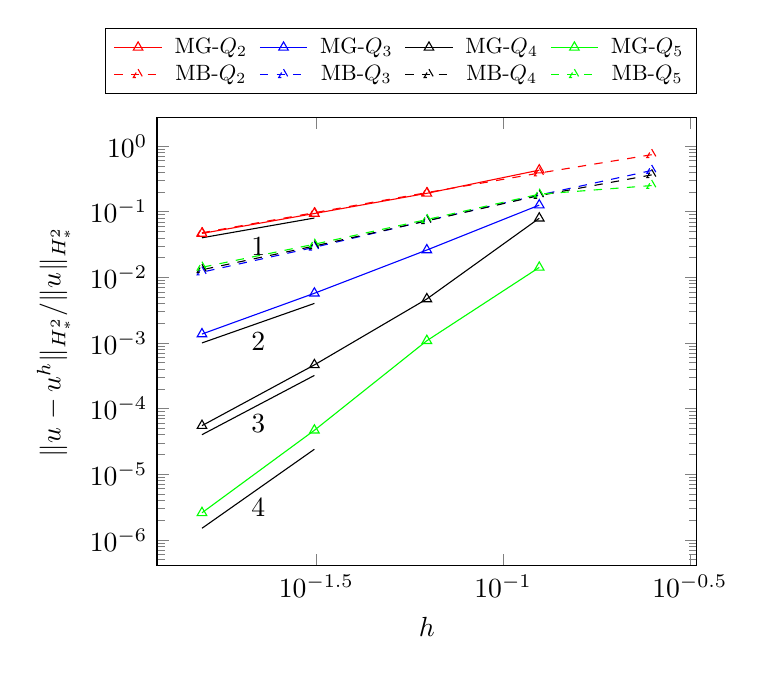
\begin{tikzpicture}
    \begin{loglogaxis}[
        legend columns=4,
    	legend style={at={(1,1.2)}, nodes={scale=0.8, transform shape}, column sep=.1cm},
        xlabel=$h$,
        ylabel=${\|u_{}-u^{h}\|_{H^2_*}}/{\|u_{}\|_{H^2_*}}$ 
    ]


    \addplot [color=red,mark=triangle] plot coordinates {


        (.125,   0.429158)
        (.0625,   0.190387)
        (0.03125,   0.0937169)
        (0.015625,  0.0465883)
    };

    
    \addplot [color=blue,mark=triangle] plot coordinates {


        (.125,      0.125872)
        (.0625,     0.0260387)
        (0.03125,   0.00570847)
        (0.015625,  0.00136665)
    };

    \addplot [color=black,mark=triangle] plot coordinates {


        (.125,      0.0794173)
        (.0625,     0.00467507)
        (0.03125,   0.000462874)
        (0.015625,  5.49137e-05)
    };

    \addplot [color=green,mark=triangle] plot coordinates {


        (.125,      0.0141393)
        (.0625,     0.00108092)
        (0.03125,   4.67021e-05)
        (0.015625,  2.58318e-06)
    };

    
    \addplot [color=red,mark=triangle, dashed] plot coordinates {

        (.25,       0.73789)
        (.125,      0.387214)
        (.0625,     0.195203)
        (0.03125,   0.0964845)
        (0.015625,  0.0476812)
    };

    \addplot [color=blue,mark=triangle, dashed] plot coordinates {


        (.25,       0.423619)
        (.125,      0.179079)
        (.0625,     0.0729287)
        (0.03125,   0.0286441)
        (0.015625,  0.0119787)
    };

    \addplot [color=black,mark=triangle, dashed] plot coordinates {


        (.25,       0.363333)
        (.125,      0.176097)
        (.0625,     0.0724466)
        (0.03125,   0.0299489)
        (0.015625,  0.0130237)
    };

    \addplot [color=green,mark=triangle, dashed] plot coordinates {


        (.25,       0.249916)
        (.125,      0.184512)
        (.0625,     0.0758842)
        (0.03125,   0.031917)
        (0.015625,  0.0142136)
    };

    \addplot [black] plot coordinates {

        (.03125,    0.08)
        (0.015625,    .04)
    } node[pos=0.5,anchor=north]{$1$};

    \addplot [black] plot coordinates {

        (.03125,    0.0040)
        (0.015625,    .001)
    } node[pos=0.5,anchor=north]{$2$};

    \addplot [black] plot coordinates {

        (.03125,    3.2000e-04)
        (0.015625,  4e-5)
    } node[pos=0.5,anchor=north]{$3$};

    \addplot [black] plot coordinates {

        (.03125,    2.4000e-05)
        (0.015625,  1.5e-6)
    } node[pos=0.5,anchor=north]{$4$};

    \legend{MG-$Q_2$\\MG-$Q_3$\\MG-$Q_4$\\MG-$Q_5$\\MB-$Q_2$\\MB-$Q_3$\\MB-$Q_4$\\MB-$Q_5$\\}
    \end{loglogaxis}
\end{tikzpicture}

\end{document}

